% Created by tikzDevice version 0.9 on 2016-01-13 23:40:07
% !TEX encoding = UTF-8 Unicode
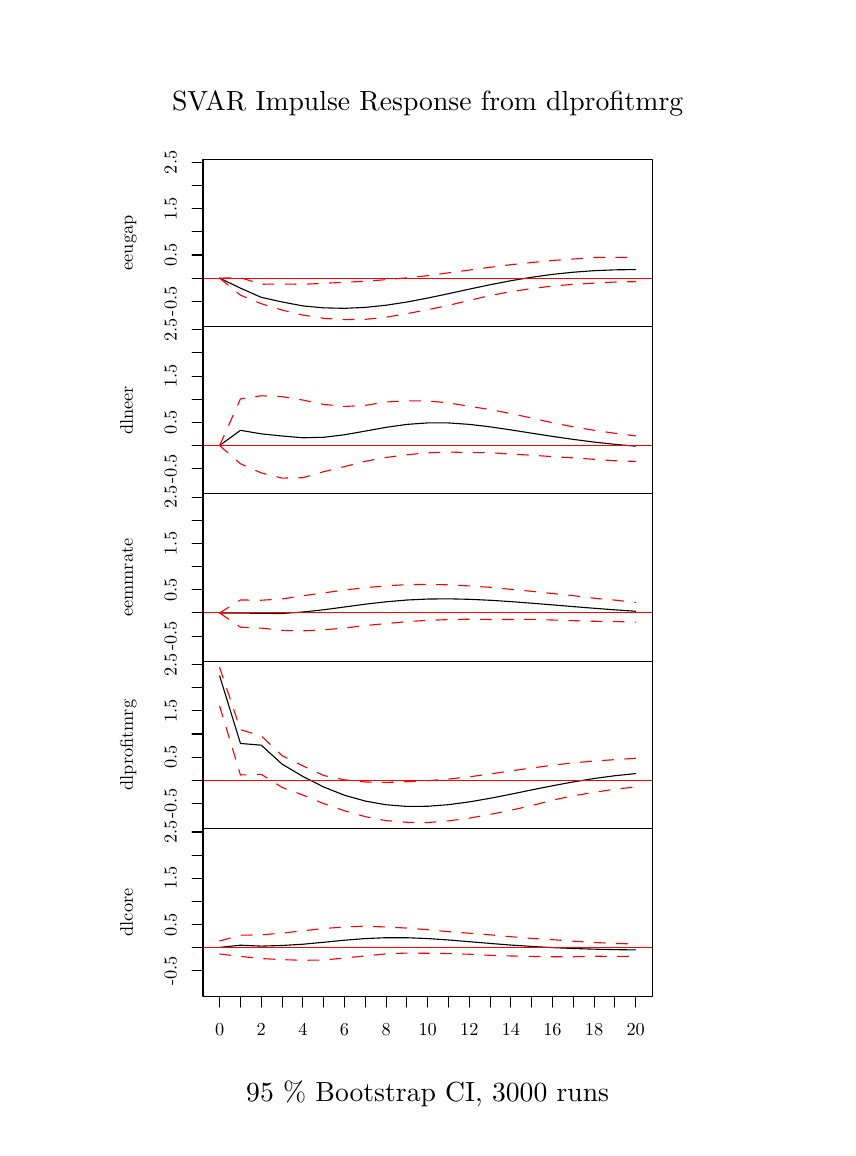
\begin{tikzpicture}[x=1pt,y=1pt]
\definecolor{fillColor}{RGB}{255,255,255}
\path[use as bounding box,fill=fillColor,fill opacity=0.00] (0,0) rectangle (289.08,397.48);
\begin{scope}
\path[clip] ( 63.36,289.48) rectangle (225.72,349.96);
\definecolor{drawColor}{RGB}{0,0,0}

\path[draw=drawColor,line width= 0.4pt,line join=round,line cap=round] ( 69.37,306.97) --
	( 76.89,303.36) --
	( 84.41,300.03) --
	( 91.92,298.37) --
	( 99.44,296.93) --
	(106.96,296.24) --
	(114.47,296.06) --
	(121.99,296.40) --
	(129.51,297.18) --
	(137.02,298.34) --
	(144.54,299.77) --
	(152.06,301.35) --
	(159.57,302.99) --
	(167.09,304.58) --
	(174.61,306.03) --
	(182.12,307.29) --
	(189.64,308.33) --
	(197.16,309.11) --
	(204.67,309.66) --
	(212.19,309.97) --
	(219.71,310.07);
\end{scope}
\begin{scope}
\path[clip] ( 31.68,289.48) rectangle (257.40,349.96);
\definecolor{drawColor}{RGB}{0,0,0}

\node[text=drawColor,anchor=base,inner sep=0pt, outer sep=0pt, scale=  0.66] at (144.54,259.38) {xy{\$}x};

\node[text=drawColor,rotate= 90.00,anchor=base,inner sep=0pt, outer sep=0pt, scale=  0.66] at ( 38.02,319.72) {eeugap};
\end{scope}
\begin{scope}
\path[clip] (  0.00,  0.00) rectangle (289.08,397.48);
\definecolor{drawColor}{RGB}{0,0,0}

\path[draw=drawColor,line width= 0.4pt,line join=round,line cap=round] ( 63.36,298.60) -- ( 63.36,348.81);

\path[draw=drawColor,line width= 0.4pt,line join=round,line cap=round] ( 63.36,298.60) -- ( 59.40,298.60);

\path[draw=drawColor,line width= 0.4pt,line join=round,line cap=round] ( 63.36,306.97) -- ( 59.40,306.97);

\path[draw=drawColor,line width= 0.4pt,line join=round,line cap=round] ( 63.36,315.34) -- ( 59.40,315.34);

\path[draw=drawColor,line width= 0.4pt,line join=round,line cap=round] ( 63.36,323.70) -- ( 59.40,323.70);

\path[draw=drawColor,line width= 0.4pt,line join=round,line cap=round] ( 63.36,332.07) -- ( 59.40,332.07);

\path[draw=drawColor,line width= 0.4pt,line join=round,line cap=round] ( 63.36,340.44) -- ( 59.40,340.44);

\path[draw=drawColor,line width= 0.4pt,line join=round,line cap=round] ( 63.36,348.81) -- ( 59.40,348.81);

\node[text=drawColor,rotate= 90.00,anchor=base,inner sep=0pt, outer sep=0pt, scale=  0.66] at ( 53.86,298.60) {-0.5};

\node[text=drawColor,rotate= 90.00,anchor=base,inner sep=0pt, outer sep=0pt, scale=  0.66] at ( 53.86,315.34) {0.5};

\node[text=drawColor,rotate= 90.00,anchor=base,inner sep=0pt, outer sep=0pt, scale=  0.66] at ( 53.86,332.07) {1.5};

\node[text=drawColor,rotate= 90.00,anchor=base,inner sep=0pt, outer sep=0pt, scale=  0.66] at ( 53.86,348.81) {2.5};
\end{scope}
\begin{scope}
\path[clip] ( 63.36,289.48) rectangle (225.72,349.96);
\definecolor{drawColor}{RGB}{255,0,0}

\path[draw=drawColor,line width= 0.4pt,line join=round,line cap=round] ( 63.36,306.97) -- (225.72,306.97);

\path[draw=drawColor,line width= 0.4pt,dash pattern=on 4pt off 4pt ,line join=round,line cap=round] ( 69.37,306.97) --
	( 76.89,307.14) --
	( 84.41,304.77) --
	( 91.92,304.83) --
	( 99.44,304.75) --
	(106.96,305.08) --
	(114.47,305.49) --
	(121.99,305.83) --
	(129.51,306.42) --
	(137.02,307.09) --
	(144.54,307.86) --
	(152.06,308.89) --
	(159.57,309.89) --
	(167.09,310.89) --
	(174.61,311.83) --
	(182.12,312.62) --
	(189.64,313.36) --
	(197.16,313.88) --
	(204.67,314.43) --
	(212.19,314.46) --
	(219.71,314.42);

\path[draw=drawColor,line width= 0.4pt,dash pattern=on 4pt off 4pt ,line join=round,line cap=round] ( 69.37,306.97) --
	( 76.89,300.81) --
	( 84.41,297.73) --
	( 91.92,295.45) --
	( 99.44,293.60) --
	(106.96,292.46) --
	(114.47,291.98) --
	(121.99,292.08) --
	(129.51,292.84) --
	(137.02,294.13) --
	(144.54,295.56) --
	(152.06,297.12) --
	(159.57,298.93) --
	(167.09,300.69) --
	(174.61,302.08) --
	(182.12,303.19) --
	(189.64,304.11) --
	(197.16,304.72) --
	(204.67,305.16) --
	(212.19,305.56) --
	(219.71,305.70);
\end{scope}
\begin{scope}
\path[clip] (  0.00,  0.00) rectangle (289.08,397.48);
\definecolor{drawColor}{RGB}{0,0,0}

\path[draw=drawColor,line width= 0.4pt,line join=round,line cap=round] ( 63.36,289.48) --
	(225.72,289.48) --
	(225.72,349.96) --
	( 63.36,349.96) --
	( 63.36,289.48);
\end{scope}
\begin{scope}
\path[clip] ( 63.36,228.99) rectangle (225.72,289.48);
\definecolor{drawColor}{RGB}{0,0,0}

\path[draw=drawColor,line width= 0.4pt,line join=round,line cap=round] ( 69.37,246.48) --
	( 76.89,251.98) --
	( 84.41,250.70) --
	( 91.92,249.93) --
	( 99.44,249.29) --
	(106.96,249.46) --
	(114.47,250.37) --
	(121.99,251.70) --
	(129.51,253.06) --
	(137.02,254.12) --
	(144.54,254.66) --
	(152.06,254.65) --
	(159.57,254.13) --
	(167.09,253.24) --
	(174.61,252.13) --
	(182.12,250.94) --
	(189.64,249.78) --
	(197.16,248.70) --
	(204.67,247.74) --
	(212.19,246.92) --
	(219.71,246.24);
\end{scope}
\begin{scope}
\path[clip] ( 31.68,228.99) rectangle (257.40,289.48);
\definecolor{drawColor}{RGB}{0,0,0}

\node[text=drawColor,anchor=base,inner sep=0pt, outer sep=0pt, scale=  0.66] at (144.54,198.89) {xy{\$}x};

\node[text=drawColor,rotate= 90.00,anchor=base,inner sep=0pt, outer sep=0pt, scale=  0.66] at ( 38.02,259.23) {dlneer};
\end{scope}
\begin{scope}
\path[clip] (  0.00,  0.00) rectangle (289.08,397.48);
\definecolor{drawColor}{RGB}{0,0,0}

\path[draw=drawColor,line width= 0.4pt,line join=round,line cap=round] ( 63.36,238.11) -- ( 63.36,288.32);

\path[draw=drawColor,line width= 0.4pt,line join=round,line cap=round] ( 63.36,238.11) -- ( 59.40,238.11);

\path[draw=drawColor,line width= 0.4pt,line join=round,line cap=round] ( 63.36,246.48) -- ( 59.40,246.48);

\path[draw=drawColor,line width= 0.4pt,line join=round,line cap=round] ( 63.36,254.85) -- ( 59.40,254.85);

\path[draw=drawColor,line width= 0.4pt,line join=round,line cap=round] ( 63.36,263.21) -- ( 59.40,263.21);

\path[draw=drawColor,line width= 0.4pt,line join=round,line cap=round] ( 63.36,271.58) -- ( 59.40,271.58);

\path[draw=drawColor,line width= 0.4pt,line join=round,line cap=round] ( 63.36,279.95) -- ( 59.40,279.95);

\path[draw=drawColor,line width= 0.4pt,line join=round,line cap=round] ( 63.36,288.32) -- ( 59.40,288.32);

\node[text=drawColor,rotate= 90.00,anchor=base,inner sep=0pt, outer sep=0pt, scale=  0.66] at ( 53.86,238.11) {-0.5};

\node[text=drawColor,rotate= 90.00,anchor=base,inner sep=0pt, outer sep=0pt, scale=  0.66] at ( 53.86,254.85) {0.5};

\node[text=drawColor,rotate= 90.00,anchor=base,inner sep=0pt, outer sep=0pt, scale=  0.66] at ( 53.86,271.58) {1.5};

\node[text=drawColor,rotate= 90.00,anchor=base,inner sep=0pt, outer sep=0pt, scale=  0.66] at ( 53.86,288.32) {2.5};
\end{scope}
\begin{scope}
\path[clip] ( 63.36,228.99) rectangle (225.72,289.48);
\definecolor{drawColor}{RGB}{255,0,0}

\path[draw=drawColor,line width= 0.4pt,line join=round,line cap=round] ( 63.36,246.48) -- (225.72,246.48);

\path[draw=drawColor,line width= 0.4pt,dash pattern=on 4pt off 4pt ,line join=round,line cap=round] ( 69.37,246.48) --
	( 76.89,263.33) --
	( 84.41,264.46) --
	( 91.92,264.15) --
	( 99.44,262.92) --
	(106.96,261.34) --
	(114.47,260.60) --
	(121.99,261.00) --
	(129.51,262.21) --
	(137.02,262.62) --
	(144.54,262.58) --
	(152.06,261.90) --
	(159.57,260.66) --
	(167.09,259.49) --
	(174.61,258.02) --
	(182.12,256.42) --
	(189.64,254.71) --
	(197.16,253.24) --
	(204.67,251.98) --
	(212.19,250.92) --
	(219.71,249.97);

\path[draw=drawColor,line width= 0.4pt,dash pattern=on 4pt off 4pt ,line join=round,line cap=round] ( 69.37,246.48) --
	( 76.89,239.90) --
	( 84.41,236.59) --
	( 91.92,234.71) --
	( 99.44,234.85) --
	(106.96,237.03) --
	(114.47,238.86) --
	(121.99,240.79) --
	(129.51,242.17) --
	(137.02,243.13) --
	(144.54,243.86) --
	(152.06,244.13) --
	(159.57,243.94) --
	(167.09,243.88) --
	(174.61,243.41) --
	(182.12,242.98) --
	(189.64,242.48) --
	(197.16,242.02) --
	(204.67,241.50) --
	(212.19,240.98) --
	(219.71,240.75);
\end{scope}
\begin{scope}
\path[clip] (  0.00,  0.00) rectangle (289.08,397.48);
\definecolor{drawColor}{RGB}{0,0,0}

\path[draw=drawColor,line width= 0.4pt,line join=round,line cap=round] ( 63.36,228.99) --
	(225.72,228.99) --
	(225.72,289.48) --
	( 63.36,289.48) --
	( 63.36,228.99);
\end{scope}
\begin{scope}
\path[clip] ( 63.36,168.50) rectangle (225.72,228.99);
\definecolor{drawColor}{RGB}{0,0,0}

\path[draw=drawColor,line width= 0.4pt,line join=round,line cap=round] ( 69.37,185.99) --
	( 76.89,185.96) --
	( 84.41,185.83) --
	( 91.92,185.79) --
	( 99.44,186.33) --
	(106.96,187.13) --
	(114.47,188.14) --
	(121.99,189.15) --
	(129.51,190.02) --
	(137.02,190.66) --
	(144.54,191.01) --
	(152.06,191.09) --
	(159.57,190.92) --
	(167.09,190.57) --
	(174.61,190.08) --
	(182.12,189.51) --
	(189.64,188.90) --
	(197.16,188.28) --
	(204.67,187.68) --
	(212.19,187.11) --
	(219.71,186.60);
\end{scope}
\begin{scope}
\path[clip] ( 31.68,168.50) rectangle (257.40,228.99);
\definecolor{drawColor}{RGB}{0,0,0}

\node[text=drawColor,anchor=base,inner sep=0pt, outer sep=0pt, scale=  0.66] at (144.54,138.40) {xy{\$}x};

\node[text=drawColor,rotate= 90.00,anchor=base,inner sep=0pt, outer sep=0pt, scale=  0.66] at ( 38.02,198.74) {eemmrate};
\end{scope}
\begin{scope}
\path[clip] (  0.00,  0.00) rectangle (289.08,397.48);
\definecolor{drawColor}{RGB}{0,0,0}

\path[draw=drawColor,line width= 0.4pt,line join=round,line cap=round] ( 63.36,177.62) -- ( 63.36,227.83);

\path[draw=drawColor,line width= 0.4pt,line join=round,line cap=round] ( 63.36,177.62) -- ( 59.40,177.62);

\path[draw=drawColor,line width= 0.4pt,line join=round,line cap=round] ( 63.36,185.99) -- ( 59.40,185.99);

\path[draw=drawColor,line width= 0.4pt,line join=round,line cap=round] ( 63.36,194.36) -- ( 59.40,194.36);

\path[draw=drawColor,line width= 0.4pt,line join=round,line cap=round] ( 63.36,202.73) -- ( 59.40,202.73);

\path[draw=drawColor,line width= 0.4pt,line join=round,line cap=round] ( 63.36,211.09) -- ( 59.40,211.09);

\path[draw=drawColor,line width= 0.4pt,line join=round,line cap=round] ( 63.36,219.46) -- ( 59.40,219.46);

\path[draw=drawColor,line width= 0.4pt,line join=round,line cap=round] ( 63.36,227.83) -- ( 59.40,227.83);

\node[text=drawColor,rotate= 90.00,anchor=base,inner sep=0pt, outer sep=0pt, scale=  0.66] at ( 53.86,177.62) {-0.5};

\node[text=drawColor,rotate= 90.00,anchor=base,inner sep=0pt, outer sep=0pt, scale=  0.66] at ( 53.86,194.36) {0.5};

\node[text=drawColor,rotate= 90.00,anchor=base,inner sep=0pt, outer sep=0pt, scale=  0.66] at ( 53.86,211.09) {1.5};

\node[text=drawColor,rotate= 90.00,anchor=base,inner sep=0pt, outer sep=0pt, scale=  0.66] at ( 53.86,227.83) {2.5};
\end{scope}
\begin{scope}
\path[clip] ( 63.36,168.50) rectangle (225.72,228.99);
\definecolor{drawColor}{RGB}{255,0,0}

\path[draw=drawColor,line width= 0.4pt,line join=round,line cap=round] ( 63.36,185.99) -- (225.72,185.99);

\path[draw=drawColor,line width= 0.4pt,dash pattern=on 4pt off 4pt ,line join=round,line cap=round] ( 69.37,185.99) --
	( 76.89,190.68) --
	( 84.41,190.59) --
	( 91.92,191.04) --
	( 99.44,192.21) --
	(106.96,193.24) --
	(114.47,194.24) --
	(121.99,195.14) --
	(129.51,195.76) --
	(137.02,196.24) --
	(144.54,196.30) --
	(152.06,196.15) --
	(159.57,195.75) --
	(167.09,195.25) --
	(174.61,194.52) --
	(182.12,193.80) --
	(189.64,193.01) --
	(197.16,192.22) --
	(204.67,191.31) --
	(212.19,190.62) --
	(219.71,189.80);

\path[draw=drawColor,line width= 0.4pt,dash pattern=on 4pt off 4pt ,line join=round,line cap=round] ( 69.37,185.99) --
	( 76.89,180.83) --
	( 84.41,180.51) --
	( 91.92,179.70) --
	( 99.44,179.52) --
	(106.96,179.88) --
	(114.47,180.55) --
	(121.99,181.44) --
	(129.51,182.14) --
	(137.02,182.86) --
	(144.54,183.32) --
	(152.06,183.58) --
	(159.57,183.72) --
	(167.09,183.63) --
	(174.61,183.62) --
	(182.12,183.66) --
	(189.64,183.43) --
	(197.16,183.20) --
	(204.67,182.98) --
	(212.19,182.89) --
	(219.71,182.65);
\end{scope}
\begin{scope}
\path[clip] (  0.00,  0.00) rectangle (289.08,397.48);
\definecolor{drawColor}{RGB}{0,0,0}

\path[draw=drawColor,line width= 0.4pt,line join=round,line cap=round] ( 63.36,168.50) --
	(225.72,168.50) --
	(225.72,228.99) --
	( 63.36,228.99) --
	( 63.36,168.50);
\end{scope}
\begin{scope}
\path[clip] ( 63.36,108.01) rectangle (225.72,168.50);
\definecolor{drawColor}{RGB}{0,0,0}

\path[draw=drawColor,line width= 0.4pt,line join=round,line cap=round] ( 69.37,163.24) --
	( 76.89,138.83) --
	( 84.41,138.20) --
	( 91.92,131.36) --
	( 99.44,126.91) --
	(106.96,123.10) --
	(114.47,120.11) --
	(121.99,118.01) --
	(129.51,116.68) --
	(137.02,116.08) --
	(144.54,116.13) --
	(152.06,116.71) --
	(159.57,117.71) --
	(167.09,119.01) --
	(174.61,120.49) --
	(182.12,122.04) --
	(189.64,123.54) --
	(197.16,124.94) --
	(204.67,126.16) --
	(212.19,127.17) --
	(219.71,127.94);
\end{scope}
\begin{scope}
\path[clip] ( 31.68,108.01) rectangle (257.40,168.50);
\definecolor{drawColor}{RGB}{0,0,0}

\node[text=drawColor,anchor=base,inner sep=0pt, outer sep=0pt, scale=  0.66] at (144.54, 77.91) {xy{\$}x};

\node[text=drawColor,rotate= 90.00,anchor=base,inner sep=0pt, outer sep=0pt, scale=  0.66] at ( 38.02,138.25) {dlprofitmrg};
\end{scope}
\begin{scope}
\path[clip] (  0.00,  0.00) rectangle (289.08,397.48);
\definecolor{drawColor}{RGB}{0,0,0}

\path[draw=drawColor,line width= 0.4pt,line join=round,line cap=round] ( 63.36,117.13) -- ( 63.36,167.34);

\path[draw=drawColor,line width= 0.4pt,line join=round,line cap=round] ( 63.36,117.13) -- ( 59.40,117.13);

\path[draw=drawColor,line width= 0.4pt,line join=round,line cap=round] ( 63.36,125.50) -- ( 59.40,125.50);

\path[draw=drawColor,line width= 0.4pt,line join=round,line cap=round] ( 63.36,133.87) -- ( 59.40,133.87);

\path[draw=drawColor,line width= 0.4pt,line join=round,line cap=round] ( 63.36,142.24) -- ( 59.40,142.24);

\path[draw=drawColor,line width= 0.4pt,line join=round,line cap=round] ( 63.36,150.60) -- ( 59.40,150.60);

\path[draw=drawColor,line width= 0.4pt,line join=round,line cap=round] ( 63.36,158.97) -- ( 59.40,158.97);

\path[draw=drawColor,line width= 0.4pt,line join=round,line cap=round] ( 63.36,167.34) -- ( 59.40,167.34);

\node[text=drawColor,rotate= 90.00,anchor=base,inner sep=0pt, outer sep=0pt, scale=  0.66] at ( 53.86,117.13) {-0.5};

\node[text=drawColor,rotate= 90.00,anchor=base,inner sep=0pt, outer sep=0pt, scale=  0.66] at ( 53.86,133.87) {0.5};

\node[text=drawColor,rotate= 90.00,anchor=base,inner sep=0pt, outer sep=0pt, scale=  0.66] at ( 53.86,150.60) {1.5};

\node[text=drawColor,rotate= 90.00,anchor=base,inner sep=0pt, outer sep=0pt, scale=  0.66] at ( 53.86,167.34) {2.5};
\end{scope}
\begin{scope}
\path[clip] ( 63.36,108.01) rectangle (225.72,168.50);
\definecolor{drawColor}{RGB}{255,0,0}

\path[draw=drawColor,line width= 0.4pt,line join=round,line cap=round] ( 63.36,125.50) -- (225.72,125.50);

\path[draw=drawColor,line width= 0.4pt,dash pattern=on 4pt off 4pt ,line join=round,line cap=round] ( 69.37,166.26) --
	( 76.89,143.79) --
	( 84.41,141.58) --
	( 91.92,134.40) --
	( 99.44,130.73) --
	(106.96,127.24) --
	(114.47,125.69) --
	(121.99,124.91) --
	(129.51,124.75) --
	(137.02,125.00) --
	(144.54,125.38) --
	(152.06,125.96) --
	(159.57,126.77) --
	(167.09,127.80) --
	(174.61,128.91) --
	(182.12,129.96) --
	(189.64,130.98) --
	(197.16,131.82) --
	(204.67,132.48) --
	(212.19,132.98) --
	(219.71,133.49);

\path[draw=drawColor,line width= 0.4pt,dash pattern=on 4pt off 4pt ,line join=round,line cap=round] ( 69.37,152.30) --
	( 76.89,127.44) --
	( 84.41,127.67) --
	( 91.92,122.94) --
	( 99.44,120.19) --
	(106.96,117.09) --
	(114.47,114.51) --
	(121.99,112.38) --
	(129.51,110.95) --
	(137.02,110.34) --
	(144.54,110.25) --
	(152.06,110.87) --
	(159.57,111.83) --
	(167.09,113.19) --
	(174.61,114.70) --
	(182.12,116.37) --
	(189.64,118.33) --
	(197.16,119.92) --
	(204.67,121.15) --
	(212.19,122.33) --
	(219.71,123.09);
\end{scope}
\begin{scope}
\path[clip] (  0.00,  0.00) rectangle (289.08,397.48);
\definecolor{drawColor}{RGB}{0,0,0}

\path[draw=drawColor,line width= 0.4pt,line join=round,line cap=round] ( 63.36,108.01) --
	(225.72,108.01) --
	(225.72,168.50) --
	( 63.36,168.50) --
	( 63.36,108.01);
\end{scope}
\begin{scope}
\path[clip] ( 63.36, 47.52) rectangle (225.72,108.01);
\definecolor{drawColor}{RGB}{0,0,0}

\path[draw=drawColor,line width= 0.4pt,line join=round,line cap=round] ( 69.37, 65.13) --
	( 76.89, 65.93) --
	( 84.41, 65.60) --
	( 91.92, 65.83) --
	( 99.44, 66.28) --
	(106.96, 66.99) --
	(114.47, 67.73) --
	(121.99, 68.33) --
	(129.51, 68.64) --
	(137.02, 68.63) --
	(144.54, 68.33) --
	(152.06, 67.82) --
	(159.57, 67.20) --
	(167.09, 66.57) --
	(174.61, 65.98) --
	(182.12, 65.48) --
	(189.64, 65.06) --
	(197.16, 64.74) --
	(204.67, 64.50) --
	(212.19, 64.33) --
	(219.71, 64.22);
\end{scope}
\begin{scope}
\path[clip] ( 31.68, 47.52) rectangle (257.40,108.01);
\definecolor{drawColor}{RGB}{0,0,0}

\node[text=drawColor,anchor=base,inner sep=0pt, outer sep=0pt, scale=  0.66] at (144.54, 17.42) {xy{\$}x};

\node[text=drawColor,rotate= 90.00,anchor=base,inner sep=0pt, outer sep=0pt, scale=  0.66] at ( 38.02, 77.76) {dlcore};
\end{scope}
\begin{scope}
\path[clip] (  0.00,  0.00) rectangle (289.08,397.48);
\definecolor{drawColor}{RGB}{0,0,0}

\path[draw=drawColor,line width= 0.4pt,line join=round,line cap=round] ( 63.36, 56.64) -- ( 63.36,106.85);

\path[draw=drawColor,line width= 0.4pt,line join=round,line cap=round] ( 63.36, 56.64) -- ( 59.40, 56.64);

\path[draw=drawColor,line width= 0.4pt,line join=round,line cap=round] ( 63.36, 65.01) -- ( 59.40, 65.01);

\path[draw=drawColor,line width= 0.4pt,line join=round,line cap=round] ( 63.36, 73.38) -- ( 59.40, 73.38);

\path[draw=drawColor,line width= 0.4pt,line join=round,line cap=round] ( 63.36, 81.75) -- ( 59.40, 81.75);

\path[draw=drawColor,line width= 0.4pt,line join=round,line cap=round] ( 63.36, 90.12) -- ( 59.40, 90.12);

\path[draw=drawColor,line width= 0.4pt,line join=round,line cap=round] ( 63.36, 98.48) -- ( 59.40, 98.48);

\path[draw=drawColor,line width= 0.4pt,line join=round,line cap=round] ( 63.36,106.85) -- ( 59.40,106.85);

\node[text=drawColor,rotate= 90.00,anchor=base,inner sep=0pt, outer sep=0pt, scale=  0.66] at ( 53.86, 56.64) {-0.5};

\node[text=drawColor,rotate= 90.00,anchor=base,inner sep=0pt, outer sep=0pt, scale=  0.66] at ( 53.86, 73.38) {0.5};

\node[text=drawColor,rotate= 90.00,anchor=base,inner sep=0pt, outer sep=0pt, scale=  0.66] at ( 53.86, 90.12) {1.5};

\node[text=drawColor,rotate= 90.00,anchor=base,inner sep=0pt, outer sep=0pt, scale=  0.66] at ( 53.86,106.85) {2.5};

\path[draw=drawColor,line width= 0.4pt,line join=round,line cap=round] ( 69.37, 47.52) -- (219.71, 47.52);

\path[draw=drawColor,line width= 0.4pt,line join=round,line cap=round] ( 69.37, 47.52) -- ( 69.37, 43.56);

\path[draw=drawColor,line width= 0.4pt,line join=round,line cap=round] ( 76.89, 47.52) -- ( 76.89, 43.56);

\path[draw=drawColor,line width= 0.4pt,line join=round,line cap=round] ( 84.41, 47.52) -- ( 84.41, 43.56);

\path[draw=drawColor,line width= 0.4pt,line join=round,line cap=round] ( 91.92, 47.52) -- ( 91.92, 43.56);

\path[draw=drawColor,line width= 0.4pt,line join=round,line cap=round] ( 99.44, 47.52) -- ( 99.44, 43.56);

\path[draw=drawColor,line width= 0.4pt,line join=round,line cap=round] (106.96, 47.52) -- (106.96, 43.56);

\path[draw=drawColor,line width= 0.4pt,line join=round,line cap=round] (114.47, 47.52) -- (114.47, 43.56);

\path[draw=drawColor,line width= 0.4pt,line join=round,line cap=round] (121.99, 47.52) -- (121.99, 43.56);

\path[draw=drawColor,line width= 0.4pt,line join=round,line cap=round] (129.51, 47.52) -- (129.51, 43.56);

\path[draw=drawColor,line width= 0.4pt,line join=round,line cap=round] (137.02, 47.52) -- (137.02, 43.56);

\path[draw=drawColor,line width= 0.4pt,line join=round,line cap=round] (144.54, 47.52) -- (144.54, 43.56);

\path[draw=drawColor,line width= 0.4pt,line join=round,line cap=round] (152.06, 47.52) -- (152.06, 43.56);

\path[draw=drawColor,line width= 0.4pt,line join=round,line cap=round] (159.57, 47.52) -- (159.57, 43.56);

\path[draw=drawColor,line width= 0.4pt,line join=round,line cap=round] (167.09, 47.52) -- (167.09, 43.56);

\path[draw=drawColor,line width= 0.4pt,line join=round,line cap=round] (174.61, 47.52) -- (174.61, 43.56);

\path[draw=drawColor,line width= 0.4pt,line join=round,line cap=round] (182.12, 47.52) -- (182.12, 43.56);

\path[draw=drawColor,line width= 0.4pt,line join=round,line cap=round] (189.64, 47.52) -- (189.64, 43.56);

\path[draw=drawColor,line width= 0.4pt,line join=round,line cap=round] (197.16, 47.52) -- (197.16, 43.56);

\path[draw=drawColor,line width= 0.4pt,line join=round,line cap=round] (204.67, 47.52) -- (204.67, 43.56);

\path[draw=drawColor,line width= 0.4pt,line join=round,line cap=round] (212.19, 47.52) -- (212.19, 43.56);

\path[draw=drawColor,line width= 0.4pt,line join=round,line cap=round] (219.71, 47.52) -- (219.71, 43.56);

\node[text=drawColor,anchor=base,inner sep=0pt, outer sep=0pt, scale=  0.66] at ( 69.37, 33.26) {0};

\node[text=drawColor,anchor=base,inner sep=0pt, outer sep=0pt, scale=  0.66] at ( 84.41, 33.26) {2};

\node[text=drawColor,anchor=base,inner sep=0pt, outer sep=0pt, scale=  0.66] at ( 99.44, 33.26) {4};

\node[text=drawColor,anchor=base,inner sep=0pt, outer sep=0pt, scale=  0.66] at (114.47, 33.26) {6};

\node[text=drawColor,anchor=base,inner sep=0pt, outer sep=0pt, scale=  0.66] at (129.51, 33.26) {8};

\node[text=drawColor,anchor=base,inner sep=0pt, outer sep=0pt, scale=  0.66] at (144.54, 33.26) {10};

\node[text=drawColor,anchor=base,inner sep=0pt, outer sep=0pt, scale=  0.66] at (159.57, 33.26) {12};

\node[text=drawColor,anchor=base,inner sep=0pt, outer sep=0pt, scale=  0.66] at (174.61, 33.26) {14};

\node[text=drawColor,anchor=base,inner sep=0pt, outer sep=0pt, scale=  0.66] at (189.64, 33.26) {16};

\node[text=drawColor,anchor=base,inner sep=0pt, outer sep=0pt, scale=  0.66] at (204.67, 33.26) {18};

\node[text=drawColor,anchor=base,inner sep=0pt, outer sep=0pt, scale=  0.66] at (219.71, 33.26) {20};

\path[draw=drawColor,line width= 0.4pt,line join=round,line cap=round] ( 63.36, 47.52) --
	(225.72, 47.52) --
	(225.72,108.01) --
	( 63.36,108.01) --
	( 63.36, 47.52);
\end{scope}
\begin{scope}
\path[clip] ( 63.36, 47.52) rectangle (225.72,108.01);
\definecolor{drawColor}{RGB}{255,0,0}

\path[draw=drawColor,line width= 0.4pt,line join=round,line cap=round] ( 63.36, 65.01) -- (225.72, 65.01);

\path[draw=drawColor,line width= 0.4pt,dash pattern=on 4pt off 4pt ,line join=round,line cap=round] ( 69.37, 67.46) --
	( 76.89, 69.54) --
	( 84.41, 69.66) --
	( 91.92, 70.30) --
	( 99.44, 71.12) --
	(106.96, 71.95) --
	(114.47, 72.52) --
	(121.99, 72.82) --
	(129.51, 72.50) --
	(137.02, 72.12) --
	(144.54, 71.52) --
	(152.06, 70.83) --
	(159.57, 70.27) --
	(167.09, 69.68) --
	(174.61, 69.00) --
	(182.12, 68.38) --
	(189.64, 67.92) --
	(197.16, 67.39) --
	(204.67, 66.91) --
	(212.19, 66.58) --
	(219.71, 66.35);

\path[draw=drawColor,line width= 0.4pt,dash pattern=on 4pt off 4pt ,line join=round,line cap=round] ( 69.37, 62.75) --
	( 76.89, 61.89) --
	( 84.41, 61.10) --
	( 91.92, 60.71) --
	( 99.44, 60.48) --
	(106.96, 60.58) --
	(114.47, 61.30) --
	(121.99, 62.05) --
	(129.51, 62.80) --
	(137.02, 63.09) --
	(144.54, 63.01) --
	(152.06, 62.90) --
	(159.57, 62.67) --
	(167.09, 62.27) --
	(174.61, 62.04) --
	(182.12, 61.88) --
	(189.64, 61.77) --
	(197.16, 61.77) --
	(204.67, 61.93) --
	(212.19, 61.90) --
	(219.71, 61.93);
\end{scope}
\begin{scope}
\path[clip] (  0.00,  0.00) rectangle (289.08,397.48);
\definecolor{drawColor}{RGB}{0,0,0}

\node[text=drawColor,anchor=base,inner sep=0pt, outer sep=0pt, scale=  1.00] at (144.54,367.39) {SVAR Impulse Response from dlprofitmrg};

\node[text=drawColor,anchor=base,inner sep=0pt, outer sep=0pt, scale=  1.00] at (144.54,  9.50) {95 {\%} Bootstrap CI,  3000 runs};
\end{scope}
\end{tikzpicture}
